\documentclass{standalone}
\usepackage{tikz}
\usetikzlibrary{arrows,mindmap,shapes,positioning,shadows,trees}

\tikzset{
	basic/.style  = {concept, text width=2cm, drop shadow, font=\sffamily},
  root/.append style   = {concept, fill=green!30, thin, align=center},
  level 2/.style = {basic, thin,align=center, fill=green!60},
  level 3/.style = {basic, align=left, fill=pink!60}
}

\begin{document}
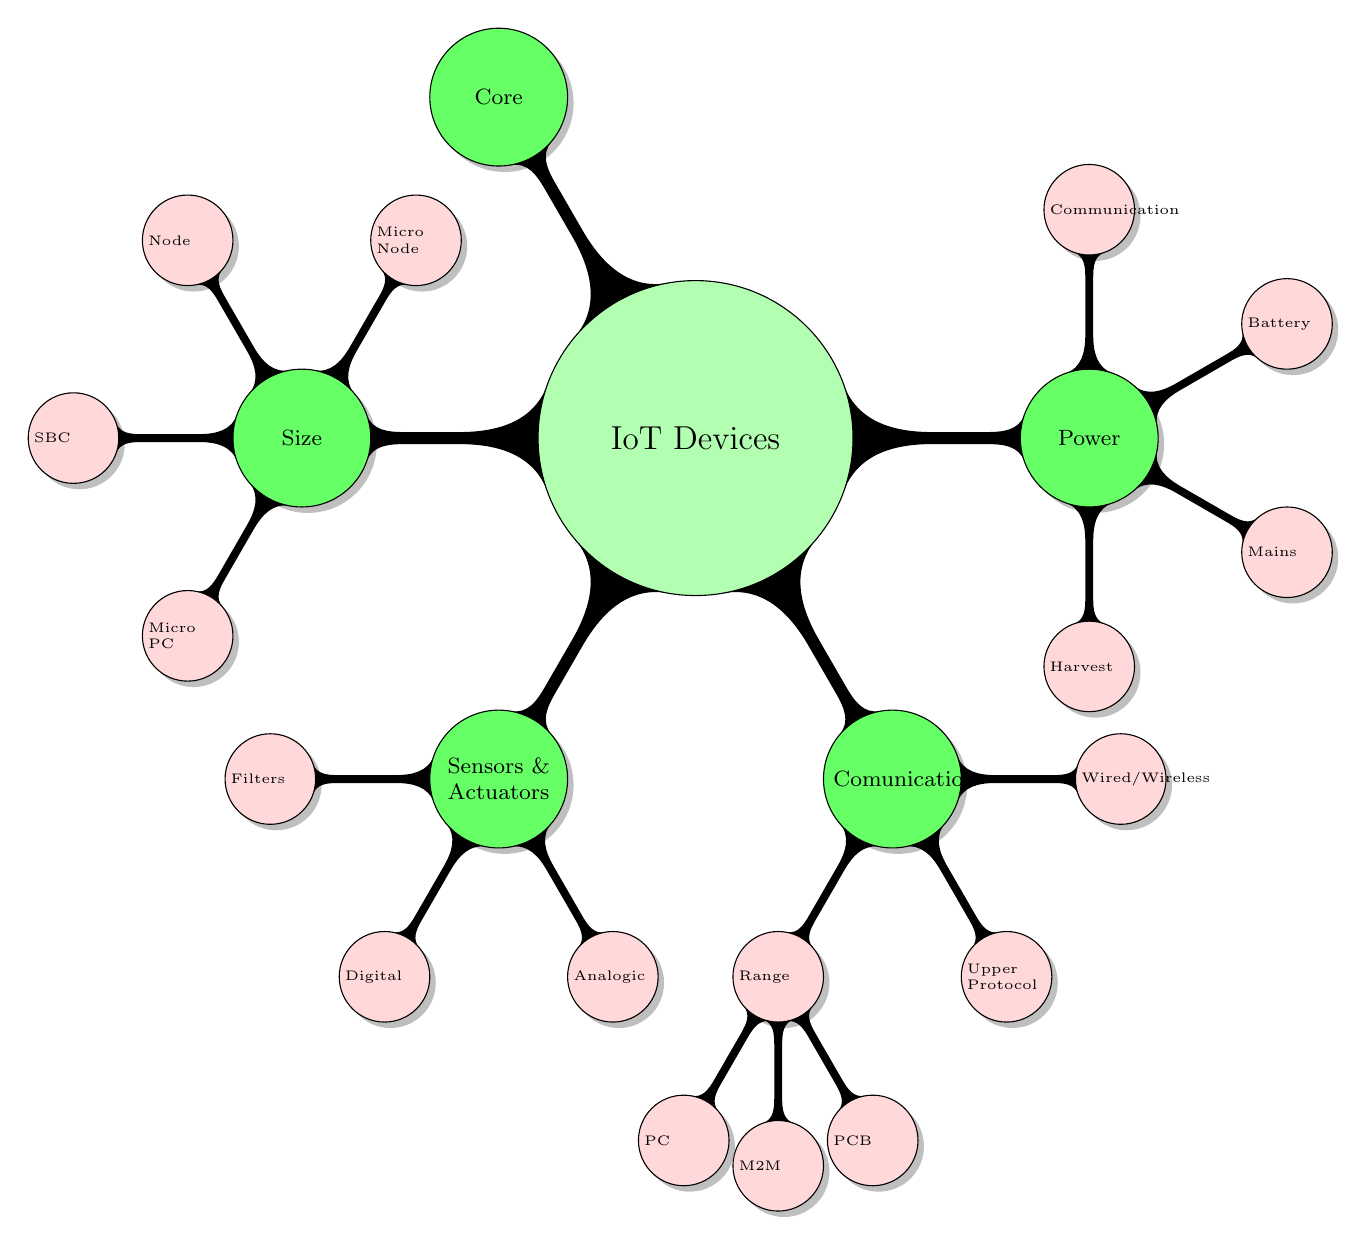
\begin{tikzpicture}
[clockwise from=0,
  level 1/.style={sibling distance=40mm},
 % edge from parent/.style={->,draw},
   mindmap]

% root of the the initial tree, level 1
\node[root] {IoT Devices}
% The first level, as children of the initial tree
  child {node[level 2] (c1) {Power}
  	[clockwise from =90]
    child{ node [level 3] (c11) {Communication}}
  	child{ node [level 3] (c12) {Battery}}
  	child{ node [level 3] (c13) {Mains}}
  	child{ node [level 3] (c14) {Harvest}}
    }
  child {node[level 2] (c2) {Comunication}
	child{node [level 3] (c21) {Wired/Wireless}}	
	child{ node [level 3] (c22) {Upper Protocol}}
	child{ node [level 3] (c23) {Range}
		[clockwise from =-60]
		child{ node[level 3] (c231){PCB}}
		child{ node[level 3] (c232){M2M}}
		child{ node[level 3] (c233){PC}}  
    }
  }
  child {node[level 2] (c3) {Sensors \& Actuators}
  	[clockwise from =-60]
  	child {node [level 3] (c31) {Analogic}}
  	child {node [level 3] (c32) {Digital}}
    child {node [level 3] (c33) {Filters}}
  }
  child {node[level 2] (c4) {Size}
  	[clockwise from =-120]
  	child {node [level 3] (c41) {Micro PC}}
  	child {node [level 3] (c42) {SBC}}
  	child {node [level 3] (c43) {Node}}
  	child {node [level 3] (c44) {Micro Node}}
  }
  child {node[level 2] (c5) {Core}};

% lines from each level 1 node to every one of its "children"

\end{tikzpicture}
\end{document}
